
\فصل{کارهای پیشین}
\قسمت{الگوریتم‌های کوانتومی در هندسهٔ محاسباتی}

استفاده از ابزارِ رایانشِ کوانتومی در هندسهٔ محاسباتی از بدوِ پیدایشِ این شاخه و توسعهٔ الگوریتم‌های مشهورِ آن، موردِ بررسی قرار گرفته \مرجع{sadakane2001}\مرجع{sadakane2002} اما با این‌حال تا امروزه ادبیاتِ کاملاً محدودی وجود دارد که الگوریتم‌ها و حدهایی در آن به صورتِ‌ موردی بررسی شده‌اند. هرچند تعدادِ این حدود و الگوریتم‌ها کم نیست اما هنوز تلاش‌ها در جهتِ تعمیم و کلیت‌بخشی به این گزاره‌ها چندان زیاد نبوده‌اند.

همچنین نکتهٔ مهمی که حائزِ اهمیتِ بیشتری‌ست این است که بیشترِ تلاش‌ها در این حوزه معطوف به استفاده از الگوریتم‌های جست‌وجو، شمارش و یا ولگشت‌های کوانتومی هستند که بهبودِ سرعتِ آن‌ها در نهایت می‌تواند به شکلِ مربعی باشد. و به نظر می‌رسد هنوز از الگوریتم‌هایی که بهبودِ سرعتِ توانی
 دارند در این حوزه استفاده‌ای نشده‌است. 
 %\مرجع{bahadur}
 \مرجع{volpato}\مرجع{lanzagorta}\مرجع{ambainis2020}\مرجع{buhrman}

در ادامه به بررسیِ الگوریتم‌ها و حدود در تلاش‌های پیشین می‌پردازیم.

از آن‌جا که هدف از این بررسی‌ها، بستگیِ پیچیدگیِ محاسباتی به پارامترهایی نظیرِ بعد و دقتِ ارقام نیست، در مرتبهٔ الگوریتم‌ها و حدها ثابت فرض شده‌اند و نوشته‌نشده‌اند.

\زیرقسمت{مسائلِ مربوط به تحدب}

    \متن‌سیاه{مسئلهٔ پوش محدب}: در فضای $d$-بعدی $N$ نقطه داریم، مطلوب است پوشِ محدبِ آن‌ها، یعنی چندضلعی‌ای که برابرِ مجموعهٔ همهٔ ترکیب‌های محدبِ این نقاط است. یا به عبارتی دیگر، مطلوب است مجموعه‌ای از نقاط که به شکلِ ترکیبِ محدبی از نقاطِ دیگر قابلِ نوشتن نیستند. بگیریم این پوشِ محدب $M$ رویه داشته‌باشد \مرجع{sadakane2002}\مرجع{lanzagorta}\مرجع[فصل بیست و ششم]{toth}
    \برچسب{مس:پوش-محدب}
    \شروع{فقرات}
        \فقره {الگوریتم کلاسیک}: با استفاده از برنامه‌ریزیِ خطی الگوریتمِ حساس‌به‌خروجی‌ای وجود دارد که درحالتِ غیرتبهگن
        \زیرنویس{هیچ $d+1$ نقطه‌ای وجود نداشته‌باشد که بر ابرصفحه‌ای $d-1$ بعدی قرار بگیرند.}
        در زمانِ
        $\O{N^2 + M\log N}$
        مسئله را حل می‌کند. در کلی‌ترین حالت، بهترین الگوریتمِ حساس‌به‌خروجی 
        $\O{NM}$
        و برای حالتِ دوبعدی 
        $\O{N \log M}$
        است
        \فقره {حد کلاسیک}: طبیعتاً الگوریتمِ مذکور، نیاز به زمانِ 
        $\Omega(M)$
        دارد و حدی نیز برای مقدارِ رویه‌ها وجود دارد که
        $M \le \kappa N^{\lfloor d/2 \rfloor}$
        که $\kappa$ عددی ثابت است.
        \فقره {الگوریتمِ کوانتومی}: با استفاده از تسریع در زیرروالِ برنامه‌ریزیِ خطی، در زمانِ
        $\O{M \sqrt{N} \log N}$
        قابلِ حل است که یعنی در حدِ $M$های کوچک، تسریع خواهدداشت.
        همچنین، برای حالتِ دوبعدی، با تسریع‌های مبتنی بر جست‌وجوی کوانتومی، می‌توان در زمانِ
        $\O{\sqrt{NM}}$
        این مسئله را حل کرد.
    \پایان{فقرات}

    \متن‌سیاه{مسئلهٔ محاسبهٔ فاصلهٔ هاسدورف:} فاصلهٔ هاسدورف برروی دو مجموعهٔ متراکم از نقاط به شکلِ زیر تعریف می‌شود
    \begin{equation}
        d_H(X, Y) := \max \{ \max_{x \in X} \min_{y \in Y} \norm{x - y}, \max_{y \in Y} \min_{x \in X} \norm{x - y} \}
    \end{equation}
    اگر یک $N$-ضلعیِ محدب و یک $M$-ضلعیِ محدب داشته‌باشیم، مطلوب است محاسبهٔ هاسدورفِ این دو. \مرجع{sadakane2001} \مرجع{atallah}
    \شروع{فقرات}
        \فقره {الگوریتم کلاسیک}: در زمانِ 
        $\O{M + N}$
        قابلِ حل است.
        \فقره {الگوریتمِ کوانتومی}: در زمانِ
        $\O{(N+M)^{\frac{3}{4}} \log^2 (N+M)}$
        قابلِ حل است.
    \پایان{فقرات}
    
    \متن‌سیاه{مسئلهٔ کوچک‌ترین توپِ شامل}: در فضای $d$-بعدی $N$ نقطه داریم، مطلوب است یافتنِ ابرکره‌ای $d$-بعدی با کوچک‌ترین شعاعِ ممکن که همهٔ نقاط داخلِ آن قرار بگیرند.\مرجع[فصل چهارم]{berg}\مرجع{volpato}
    \برچسب{مس:توپ-شامل}

    \شروع{فقرات}
        \فقره {الگوریتمِ کلاسیک}: در فضای دوبعدی با اضافه‌کردنِ تدریجیِ نقاط، با امیدریاضیِ زمانِ
        $\Theta(N)$
        این مسئله حل می‌شود. این الگوریتم که قابلِ تعمیم به همهٔ مسئله‌های بهینه‌سازیِ 
        \lr{LP-type}
        است در ابعادِ بالاتر نیز به‌درستی عمل می‌کند.

        \فقره {حد کوانتومی}: با کاهشِ این مسئله به مسئلهٔ 
        \lr{OR}
        حدِ پایینِ تعدادِ پرسشِ
        $\Omega(\sqrt{N})$
        اثبات می‌شود.
    \پایان{فقرات}

    
   \متن‌سیاه{مسئلهٔ پوششِ جعبه با نوارها}: در فضای دوبعدی یک جعبه به شکلِ
    $R = [a, b] \times [c, d]$
    داده‌شده، هر نوار، به فضای بینِ دو خطِ موازی در فضا می‌گوییم. تعدادِ $N$ نوار داده‌شده‌اند، مطلوب است جوابِ این سؤال که آیا این نوارها جعبه را پوشش می‌دهند.
    
   \متن‌سیاه{پوششِ مثلث‌ها} یک مثلث و $N$ مثلث داد‌ه‌شده‌اند، سؤال این است که آیا اجتماعِ $N$ مثلث، مثلثِ اولی را می‌پوشاند.
   
   \متن‌سیاه{حفره در پوشش} $N$ مثلث داده‌شده‌اند، مسئله این است که آیا اشتراکِ این‌ها دارای حفره است یا خیر.
   
   \متن‌سیاه{پوششِ چندبارهٔ نقاط} یک نقطه، یک عددِ $t$ و $N$ نیم‌صفحه داده‌شده‌اند، مطلوب است این‌که آیا نقطه با حداقل $t$ نیم‌صفحه پوشیده‌شده است یا خیر.
   
   چهار مسئلهٔ فوق، قابلِ کاهش به سه‌جمع هستند و اصطلاحاً سه‌جمع-سخت هستند، پس حدِ $\Omega(N^{2 - o(1)})$ برای زمانِ کلاسیک و حدِ $\Omega(N^{1 - o(1)})$ برای زمانِ کوانتومیِ آن‌ها معتبر است \مرجع{buhrman} و همگی با استفاده از الگوریتمی مشابهِ سه‌نقطهٔ هم‌خط، به نامِ پوششِ کلی (تعریف شده در \رجوع{مس:سه-نقطه}) در زمانِ 
   $\O{N^{1 + o(1)}}$
   حل می‌شوند. این الگوریتم از افرازِ صفحات در روشِ تقسیم و حل و از تسریعِ جست‌وجوی کوانتومی استفاده می‌کند. \مرجع{ambainis2020}
   
\زیرقسمت{مسائلِ مربوط به برخورد و اشتراک}

    \متن‌سیاه{مسئلهٔ وجود تلاقیِ پاره‌خط‌ها}: در فضای دوبعدی، $N$ پاره‌خط داریم، مطلوب است این‌که وجود دارند دوپاره‌خطی که با هم تلاقی داشته‌باشند.\مرجع[فصل دوم]{berg}\مرجع{volpato}
    \برچسب{مس:برخورد-پاره‌خط}

    \شروع{فقرات}
        \فقره {الگوریتمِ کلاسیک}: با تکنیک‌های نظیرِ جاروبِ خطی (در بخشِ \رجوع{قس:جاروب}) متعددی می‌توان در زمانِ 
        $\O{N\log N}$
        به جوابِ مسئله رسید.

        \فقره {الگوریتمِ کوانتومی}: با کاهشِ مسئله به یکتاییِ عناصرِ کوانتومی که خود با استفاده از ولگشت‌های کوانتومی حل می‌شود، مسئله با استفاده از
        $\Theta(N^{2/3})$
        پرسش از موقعیتِ پاره‌خط‌ها حل می‌شود.
    \پایان{فقرات}

    \متن‌سیاه{مسئلهٔ وجودِ اشتراکِ اجسامِ محدب}: در فضای $d$-بعدی در نظر بگیرید که $N$ شکلِ محدب داریم، هدف فهمیدنِ این است که آیا نقطه‌ای وجود دارد که در همهٔ این‌ها مشترک باشد. \مرجع{sadakane2002}\مرجع[فصل چهل و دوم]{toth}
    \شروع{فقرات}
        \فقره {الگوریتمِ کلاسیک}: می‌دانیم برای فضای دوبعدی و با فرضِ یکی بودنِ تعدادِ اضلاعِ اشکالِ محدب، الگوریتمی با پیچیدگیِ
        $\O{N}$
        وجود دارد.
        \فقره {حدِ کلاسیک}: حداقل نیاز به بررسیِ همهٔ $N$ شکل داریم پس تعدادِ پرسش از چندضلعی‌ها 
        $\Omega(N)$
        خواهدبود.
        \فقره {الگوریتمِ کوانتومی}: با استفاده از کاهشِ مسئله به ارضاپذیریِ برنامه‌ریزیِ خطی در 
        $\O{\sqrt{N}\log N}$
        پرسشِ فاصله و مقایسه مربوط به چندضلعی‌ها قابلِ حل است.
    \پایان{فقرات}

    \متن‌سیاه{مسئلهٔ برخوردِ اجسامِ درحالتِ کلی}:
     در فضای $d$-بعدی در نظر بگیرید که $N$ شکل داریم، هدف فهمیدنِ همهٔ برخوردهای این اجسام است. فرض کنید این اجسام $M$ برخورد دارند. \مرجع{lanzagorta}
    \شروع{فقرات}
        \فقره {الگوریتمِ کلاسیک}: می‌دانیم که بدونِ استفاده از خواصِ هندسیِ فضا، این کار در 
        $\O{N^2}$
        امکان‌پذیر است.
        \فقره {الگوریتمِ کوانتومی}: با استفاده از جست‌وجوی کوانتومی و همچنان بدونِ استفاده از خواصِ هندسیِ فضا، زمانِ این کار به 
        $\O{N\sqrt{M}}$
        کاهش می‌یابد.
    \پایان{فقرات}

    \متن‌سیاه{مسئلهٔ سه‌نقطه هم‌خط} \برچسب{مس:سه-نقطه}: تعدادِ $N$ نقطه در صفحه داده‌شده‌اند، مطلوب است این‌که آیا خطی وجود دارد که از سه نقطه عبور کند یا خیر. \مرجع{ambainis2020} \مرجع{buhrman} \مرجع[فصل بیست‌وهشتم]{toth}
    \شروع{فقرات}
        \فقره {الگوریتمِ کلاسیک}:
        با بیانِ این مسئله به عنوانِ وجود مثلث با مساحتِ صفر، در زمانِ 
        $\Theta(N^2)$
        قابل انجام است.
        
        \فقره {حد کلاسیک}:
        با کاهشِ این مسئله به سه‌جمع، حدس زده‌می‌شود، نیاز به زمانِ
        $\Omega(N^{2 - o(1)})$
        وجود دارد.
        \فقره {الگوریتمِ کلاسیک}:
        با استفاده از تقسیم و حل با افرازِ صفحه و استفاده از جست‌وجوی کوانتومی، در زمانِ 
        $\O{N^{1 + o(1)}}$
        قابلِ انجام است.
        \فقره {حد کوانتومی}:
        با استفاده از حدسِ سه‌جمعِ کوانتومی، نیاز به زمانِ
        $\Omega(N^{1 - o(1)})$
        وجود دارد.
    \پایان{فقرات}
    
    \متن‌سیاه{مسئلهٔ سه خطِ هم‌نقطه} \برچسب{مس:سه-خط} تعدادِ $N$ خط در صفحه داده‌شده‌اند، مطلوب است این‌که آیا نقطه‌ای وجود دارد که محلِ برخوردِ سه خط باشد یا خیر. \مرجع{ambainis2020}

    این مسئله دوگانِ مسئلهٔ قبل است و تمامیِ الگوریتم‌ها و حدود معتبر هستند.
    
   \متن‌سیاه{جداسازِ پاره‌خط‌ها} $N$ پاره‌خطِ عمودی داده‌شده‌اند، مطلوب است که آیا خطِ افقیِ داده‌شده این خاصیت را دارد که با هیچ‌کدام تلاقی نداشته‌باشد و در هر سوی خط حداقل یک پاره‌خط باشد. (یعنی همهٔ پاره‌خط‌ها بالای خط یا پایینِ خط نباشند.)
    
   \متن‌سیاه{مشاهده‌پذیریِ پاره‌خط‌ها} $N$ پاره‌خط و دو پاره‌خطِ $s_1$ و $s_2$ داده‌شده‌اند، هدف این است که بدانیم آیا نقطه‌ای برروی $s_1$ وجود دارد که بتواند حداقل یک نقطه از $s_2$ را ببیند به این معنی که خطِ واصلشان با هیچ پاره‌خطِ دیگری تلاقی نکند.
   
    \متن‌سیاه{مشاهده‌پذیری از بی‌نهایت} $N$ پاره‌خط و پاره‌خطِ $s$ داده‌شده‌اند، هدف این است که بدانیم آیا نقطه‌ای برروی $s$ وجود دارد که از بی‌نهایت دیده‌شود، یعنی از آن بتوان نیم‌خطی تا بی‌نهایت رسم کرد. 
    
    برای سه مسئلهٔ فوق نیز، حدها و الگوریتم‌های سه نقطهٔ هم‌خط برقرار است. \مرجع{ambainis2020} \مرجع{buhrman}
    
    \متن‌سیاه{مسئلهٔ چیدمانِ ابرصفحه‌ها}: $N$ ابرصفحه در فضای $d$-بعدی داریم، مطلوب است یافتنِ فضای احاطه‌شده بینِ پوشِ این صفحات،‌ اگر $M$ تعدادِ رویه‌های آن فضا باشد.
     
    این مسئله دوگانِ مسئلهٔ پوشِ محدب (تعریف شده در \رجوع{مس:پوش-محدب}) است و مواردِ گفته‌شده در آن‌جا همچنان معتبر است. \مرجع{sadakane2002}
   
    
\زیرقسمت{مسائلِ مربوط به مجاورت}

    \متن‌سیاه{مسئلهٔ نزدیک‌ترین زوج}: 
    \(N\)
    نقطه در فضای \(d\)-بعدی و یک تابعِ فاصله 
    \(d: \mathbb{R}^d \times \mathbb{R}^d \to \mathbb{R}^+\)
    داده‌شده‌اند، مطلوب است زوجی که کم‌ترین فاصله را دارند. \مرجع[فصل پنجم]{preparata}\مرجع{volpato}\مرجع{aaronson2020}

    \شروع{فقرات}
        \فقره {الگوریتمِ کلاسیک}: با استفاده از تقسیم و حل، با 
        $\Theta(N \log N)$ 
        مقایسه (بینِ فاصلهٔ زوج‌نقاط)
        امکانِ حل وجود دارد.
        البته برای الگوریتم‌های تصادفی، الگوریتم با امیدریاضیِ تعدادِ مقایسه‌ها
        $\Theta(N)$
        ممکن است.
        \فقره {حدِ کلاسیک}: با استفاده از یکتاییِ عناصر، مقایسه‌ها باید از مرتبهٔ
        $\Omega(N \log N)$
        باشند.

        \فقره {الگوریتمِ کوانتومی}: با استفاده از کاهش (با سربارِ لگاریتمی) به الگوریتمِ پیدا کردنِ کمینهٔ کوانتومی، با
        $\Theta(N^{\frac{2}{3}} \log N)$
        پرسشِ مقایسه، مسئله حل می‌شود.
        \فقره {حد کوانتومی}: با استفاده از یکتاییِ عناصر به شکلِ کوانتومی به حدِ
        $\O{N^{\frac{2}{3}}}$
        خواهیم رسید.
    \پایان{فقرات}

    \متن‌سیاه{مسئلهٔ دورترین زوج}: 
    \(N\)
    نقطه در فضای \(d\)-بعدی و یک تابعِ فاصله 
    \(d: \mathbb{R}^d \times \mathbb{R}^d \to \mathbb{R}^+\)
    داده‌شده‌اند، مطلوب است زوجی که بیشترین فاصله را دارند.
     
    نتایجِ آن مشابهِ مسئلهٔ نزدیک‌ترین زوج هستند.\مرجع{volpato}

    \متن‌سیاه{مسئلهٔ نزدیک‌ترین زوجِ دورنگ}: 
    $N$
    نقطهٔ آبی و $M$ نقطهٔ قرمز و یک تابعِ فاصله 
    \(d: \mathbb{R}^d \times \mathbb{R}^d \to \mathbb{R}^+\)
    داده‌شده‌اند، مطلوب است زوجِ ناهم‌رنگی که کم‌ترین فاصله را دارند. \مرجع{volpato}\cite[\lr{Minimum Geometric Spanning Trees}]{kao}\مرجع{aaronson2020}

    \شروع{فقرات}
        \فقره {الگوریتمِ کلاسیک}: با استفاده از زیردرختِ پوششیِ کمینهٔ هندسی، برای فاصله‌های خاصی نظیرِ $L_1$ در زمانِ 
        $\O{(N+M) \log (N+M)}$
         امکانِ حل وجود دارد.

        با استفاده از الگوریتم‌های تصادفی نیز در زمانِ
        $\O{(NM \log N\log M)^\frac{2}{3}+N\log^2M+M\log^2N}$
        حل می‌شود.
        \فقره {حدِ کلاسیک}: چون این مسئله از مسئلهٔ نزدیک‌ترین زوج سخت‌تر است حدهای قبلی برقرار هستند.

        \فقره {الگوریتمِ کوانتومی}: به شکلِ تقریباً مشابهی با مسئلهٔ نزدیک‌ترین زوج، با تعداد پرسشِ مقایسه
        $\O{(M+N)^{\frac{2}{3}} \log (M+N)}$
        حل می‌شود.
        \فقره {حد کوانتومی}: چون این مسئله از مسئلهٔ نزدیک‌ترین زوج سخت‌تر است حدهای قبلی برقرار هستند.

    \پایان{فقرات}



\قسمت{مسئلهٔ قرارگیریِ نقطه در چندضلعی}
\برچسب{مس:نقطه-در-چندضلعی}
\متن‌سیاه{مسئلهٔ قرارگیریِ نقطه در چندضلعی}: تصور کنید در یک صفحه، نقطهٔ 
\(p\)
را داریم و \(N\)-ضلعیِ 
\(G\)
که به‌ترتیب مشتکل از نقاطِ 
\(q_0 \dots q_{N-1}\)
است. \مرجع{huang}

اگر بدونِ هیچ پیش‌پردازشی، بخواهیم برای همین یک نقطه، بودن یا نبودن داخلِ چندضلعی را به دست بیاوریم، دو ایدهٔ مشهور وجود دارد.
\متن‌سیاه{ایدهٔ نخست} این است که اگر هر نیم‌خطی از این نقطه رسم کنیم، اضلاعِ چندضلعی را در فرد نقطه قطع می‌کند اگر و تنها اگر نقطه درونِ چندضلعی باشد.

با این ایده می‌توان در مرتبهٔ 
$\Theta(N)$
مسئلهٔ مذکور را حل کرد.

\متن‌سیاه{ایدهٔ دوم} به این  این ترتیب است که اگر زاویهٔ خطِ 
\( q_i ~ q_{i+1} \)
\زیرنویس{لازم است برای حالتی که 
\( i = N \)
دقتی به خرج بدهیم که اگر جمع را به پیمانهٔ 
\( N \)
فرض کرده‌باشیم، تمامِ معادلات برای آن حالت نیز معتبر خواهندبود.}
از دید 
\( p \)
را 
\( \theta_i \)

در نظر بگیریم، همچنین به آن خط عدد \(s_i\) را نسبت دهیم که

\begin{equation}
    \begin{cases}
    s_i = 0 & \text{ %
    اگر \(p\) در سمتِ راستِ خطِ \( q_i ~ q_{i+1} \) باشد %
    } \\
    s_i = 1 & \text{ %
    اگر \(p\) در سمتِ چپِ خطِ \( q_i ~ q_{i+1} \) باشد %
    } 
    \end{cases}
\end{equation}

\شروع{شکل}[آ]
\وسط‌چین
 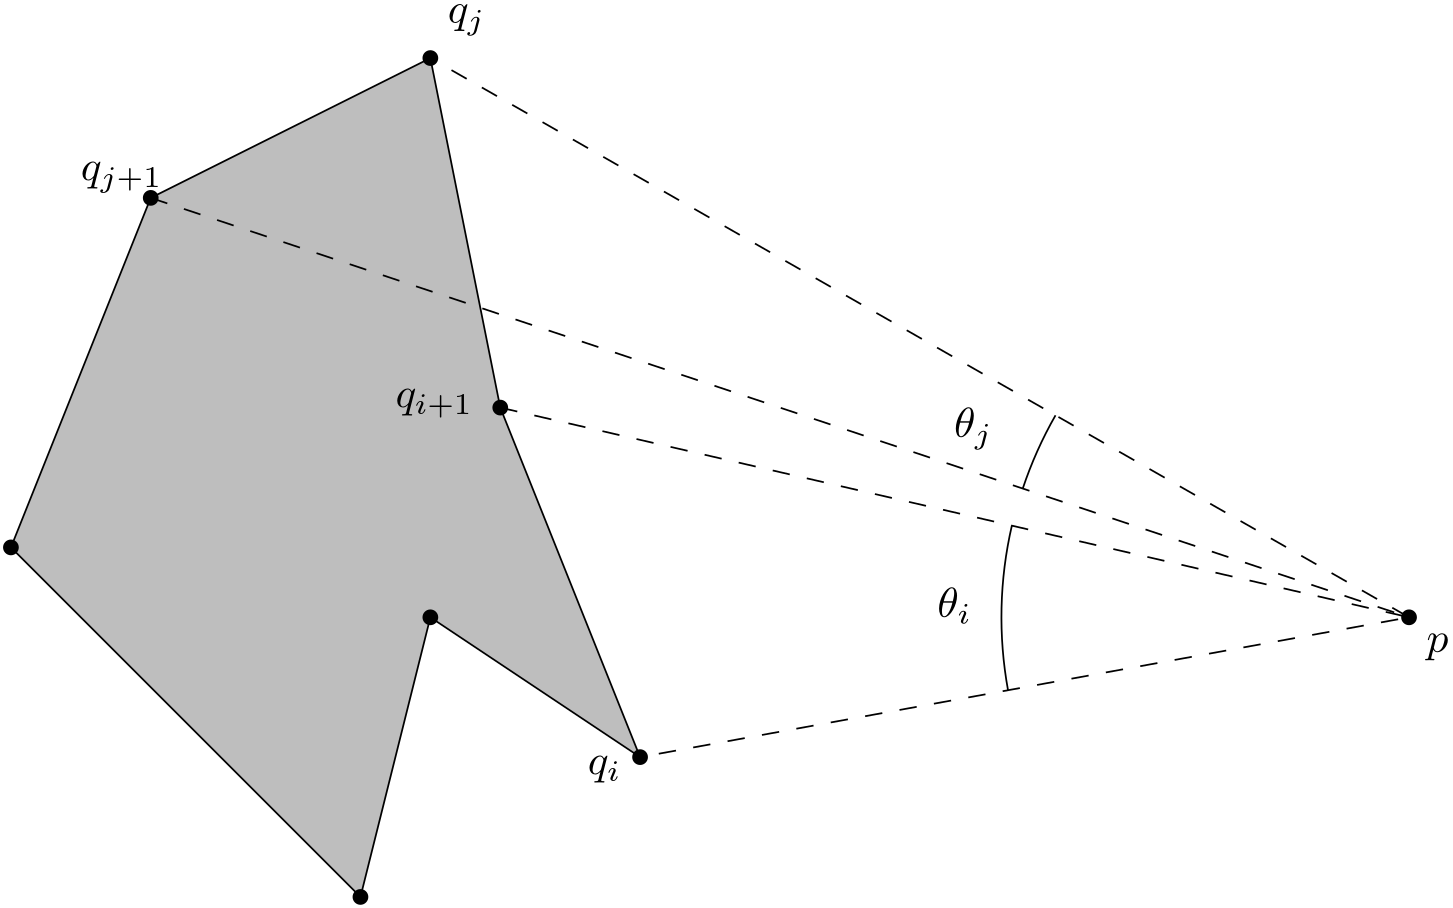
\includegraphics[width=0.8\textwidth]{figs/point-in-polygon-theta.png}
\برچسب{شکل:چندضلعی-و-زوایا}
\شرح{نمایشِ پارامترهای استفاده شده در الگوریتم}
\پایان{شکل}

حالا می‌دانیم که مسئلهٔ قرارگیریِ نقطه در چندضلعی به مسئلهٔ قولی به شکلِ زیر تبدیل می‌شود.

\begin{equation}
    \abs{\sum \theta_i s_i} = \begin{cases}
    2\pi & \text{نقطه داخلِ چندضلعی‌ست} \\
    0 & \text{نقطه بیرونِ چندضلعی‌ست}
    \end{cases}
\end{equation}

که به این شکل با این ایده در مرتبهٔ 
$\Theta(N)$
مسئلهٔ مذکور را حل کرد. البته برخلافِ ایدهٔ قبل، نیاز به محاسبهٔ توابعِ وارون‌مثلثاتی‌ست که این کار، سرعتِ این الگوریتم را در واقعیت نسبت به الگوریتمِ قبلی کاهش می‌دهد و از همین‌رو به این ترتیب استفاده نمی‌شود. اما تصحیحاتی بر این الگوریتم وجود دارد که با استفاده از تقریب‌هایی دقت را کاهش می‌دهد اما امکانِ محاسبهٔ سریع را می‌دهد.\مرجع{hormann} \مرجع{weiler}
